\appendix
\begin{comment}
\section{Erratum}\label{sec:erratum}

In our first milestone report, we presented results for baseline methods (e.g., logistic regression, SVM) evaluated on toxic comment classification tasks. However, an error in the data balancing function led to incorrect results. This erratum clarifies the error and presents corrected findings. \cite{Ammar2024}

The error occurred in the data balancing function, which ensured a specified proportion of positive examples in the dataset. The function retained all positive examples and undersampled the negative class to achieve the target ratio. However, an example was considered positive only if toxicity = 1 and negative if toxicity = 0, instead of using the correct threshold where a sample is toxic if toxicity $>$ 0.5, and non-toxic otherwise. This incorrect labeling reduced the dataset size, limiting the training data available to baseline methods. As a result, the models produced worse results that were not representative of their actual performance.
We fixed the issue by applying the correct threshold, which significantly increased the amount of training data and allowed the baseline methods to perform as expected. However, the increased dataset size introduced new computational challenges: The random forest baseline had to be removed because it was no longer computationally feasible as an ensemble method. Other methods, such as logistic regression and SVM, also required considerable time and RAM resources with the adjusted training dataset.

Corrected results presented in \cref{tab:corrected} confirm that logistic regression remains the best-performing baseline regarding F1 score for the toxic class (C1), achieving a score of 0.62 compared to the previously reported 0.52. Furthermore, preprocessing continues to yield no significant improvement, aligning with prior conclusions. Finally, baseline methods remain sensitive to class imbalance, emphasizing the need for appropriate resampling strategies. While this correction increases baseline performance, the overall findings of the first milestone remain valid. Logistic regression and SVM both perform almost equally well, preprocessing shows minimal benefit, and addressing class imbalance is critical for achieving robust performance. Most importantly, the corrected baseline F1 score of 0.62 sets a higher benchmark for our fine-tuned BERT model.

\begin{table}[h!]
    \centering
    \caption{Corrected classifier performance on the Civil Comments validation dataset}
    \label{tab:corrected}
    \resizebox{\textwidth}{!}{%
    \begin{tabular}{lccccccccc}
    \hline
    \textbf{Method}            & \textbf{Prep.} & \textbf{Pos.} & \textbf{Precision} & \textbf{Recall} & \textbf{F1} & \textbf{Macro} & \textbf{Weighted} & \textbf{Acc.} & \textbf{AUC} \\ 
                               &                        & \textbf{Prop.} & \textbf{(C1)}      & \textbf{(C1)}   & \textbf{(C1)} & \textbf{F1}   & \textbf{F1}       &               &      \textbf{ROC}            \\ \hline
    Naïve Bayes                & True                   & None          & \textbf{0.98}              & 0.06            & 0.11        & 0.54          & 0.92             & 0.95         & 0.89          \\ 
                               &                        & 0.1           & 0.93              & 0.12            & 0.21        & 0.59          & 0.93             & 0.95         & 0.89          \\ 
                               &                        & 0.25          & 0.64              & 0.43            & 0.51        & 0.74          & 0.95             & 0.95         & 0.89         \\ 
                               &                        & 0.5           & 0.19              & 0.84            & 0.31        & 0.59          & 0.84             & 0.79         & 0.89          \\ 
                               & False                  & None          & \textbf{0.98}              & 0.06            & 0.11        & 0.54          & 0.92             & 0.95         & 0.89          \\ 
                               &                        & 0.1           & 0.93              & 0.12            & 0.21        & 0.59          & 0.93             & 0.95         & 0.89          \\ 
                               &                        & 0.25          & 0.64              & 0.43            & 0.51        & 0.74          & \textbf{0.96}             & 0.95         & 0.89          \\ 
                               &                        & 0.5           & 0.19              & 0.84            & 0.32        & 0.60          & 0.84             & 0.79         & 0.89          \\ \hline
   Support Vector             & True                   & None          & 0.76              & 0.45            & 0.56        & 0.77          & 0.95             & \textbf{0.96}         & 0.93           \\ 
    Machine                    &                        & 0.1           & 0.69              & 0.54            & 0.61        & \textbf{0.79}          & \textbf{0.96}             & \textbf{0.96}         & 0.93           \\ 
                               &                        & 0.25          & 0.52              & 0.73            & 0.61        & \textbf{0.79}          & 0.95             & 0.95         & \textbf{0.94}           \\ 
                               &                        & 0.5           & 0.35              & 0.84            & 0.50        & 0.72          & 0.92             & 0.90         & \textbf{0.94}           \\ 
                               & False                  & None          & 0.76              & 0.45            & 0.56        & 0.77          & 0.95             & \textbf{0.96}         & 0.93           \\ 
                               &                        & 0.1           & 0.69              & 0.54            & 0.61        & \textbf{0.79}          & \textbf{0.96}             & \textbf{0.96}         & 0.93           \\ 
                               &                        & 0.25          & 0.52              & 0.73            & 0.61        & \textbf{0.79}          & 0.95             & 0.95         & \textbf{0.94}           \\ 
                               &                        & 0.5           & 0.35              & \textbf{0.85}            & 0.50        & 0.72          & 0.92             & 0.90         & \textbf{0.94}           \\ \hline
    Logistic                   & True                   & None           & 0.77              & 0.45            & 0.57        & 0.77          & \textbf{0.96}             & \textbf{0.96}         & 0.93           \\ 
    Regression                 &                        & 0.1          & 0.70              & 0.53            & 0.60        & \textbf{0.79}          & \textbf{0.96}             & \textbf{0.96}         & 0.93           \\ 
                     &                        & 0.25          & 0.54              & 0.71            & 0.61        & \textbf{0.79}          & 0.95             & 0.95         & \textbf{0.94}           \\ 
                               &                        & 0.5           & 0.36              & 0.84            & 0.51        & 0.73          & 0.92             & 0.91         & \textbf{0.94}           \\ 
                               & False                  & None           & 0.77              & 0.44            & 0.56        & 0.77          & 0.95             & \textbf{0.96}         & 0.93           \\ 
                               &                   & 0.1           & 0.70              & 0.53            & 0.60        & \textbf{0.79}          & \textbf{0.96}             & \textbf{0.96}         & 0.93           \\ 
                               &                        & 0.25          & 0.54              & 0.71            & \textbf{0.62}        & \textbf{0.79}          & 0.95             & 0.95         & \textbf{0.94}           \\ 
                               &                        & 0.5           & 0.37              & 0.84            & 0.52        & 0.73          & 0.92             & 0.91         & \textbf{0.94}           \\ \hline
    \end{tabular}%
    }
\end{table}
\end{comment}


\section{Confidence scores}\label{sec:confidence}

\FloatBarrier

\begin{figure}[H]
    \centering
    \begin{subfigure}[t]{0.45\textwidth}
        \centering
        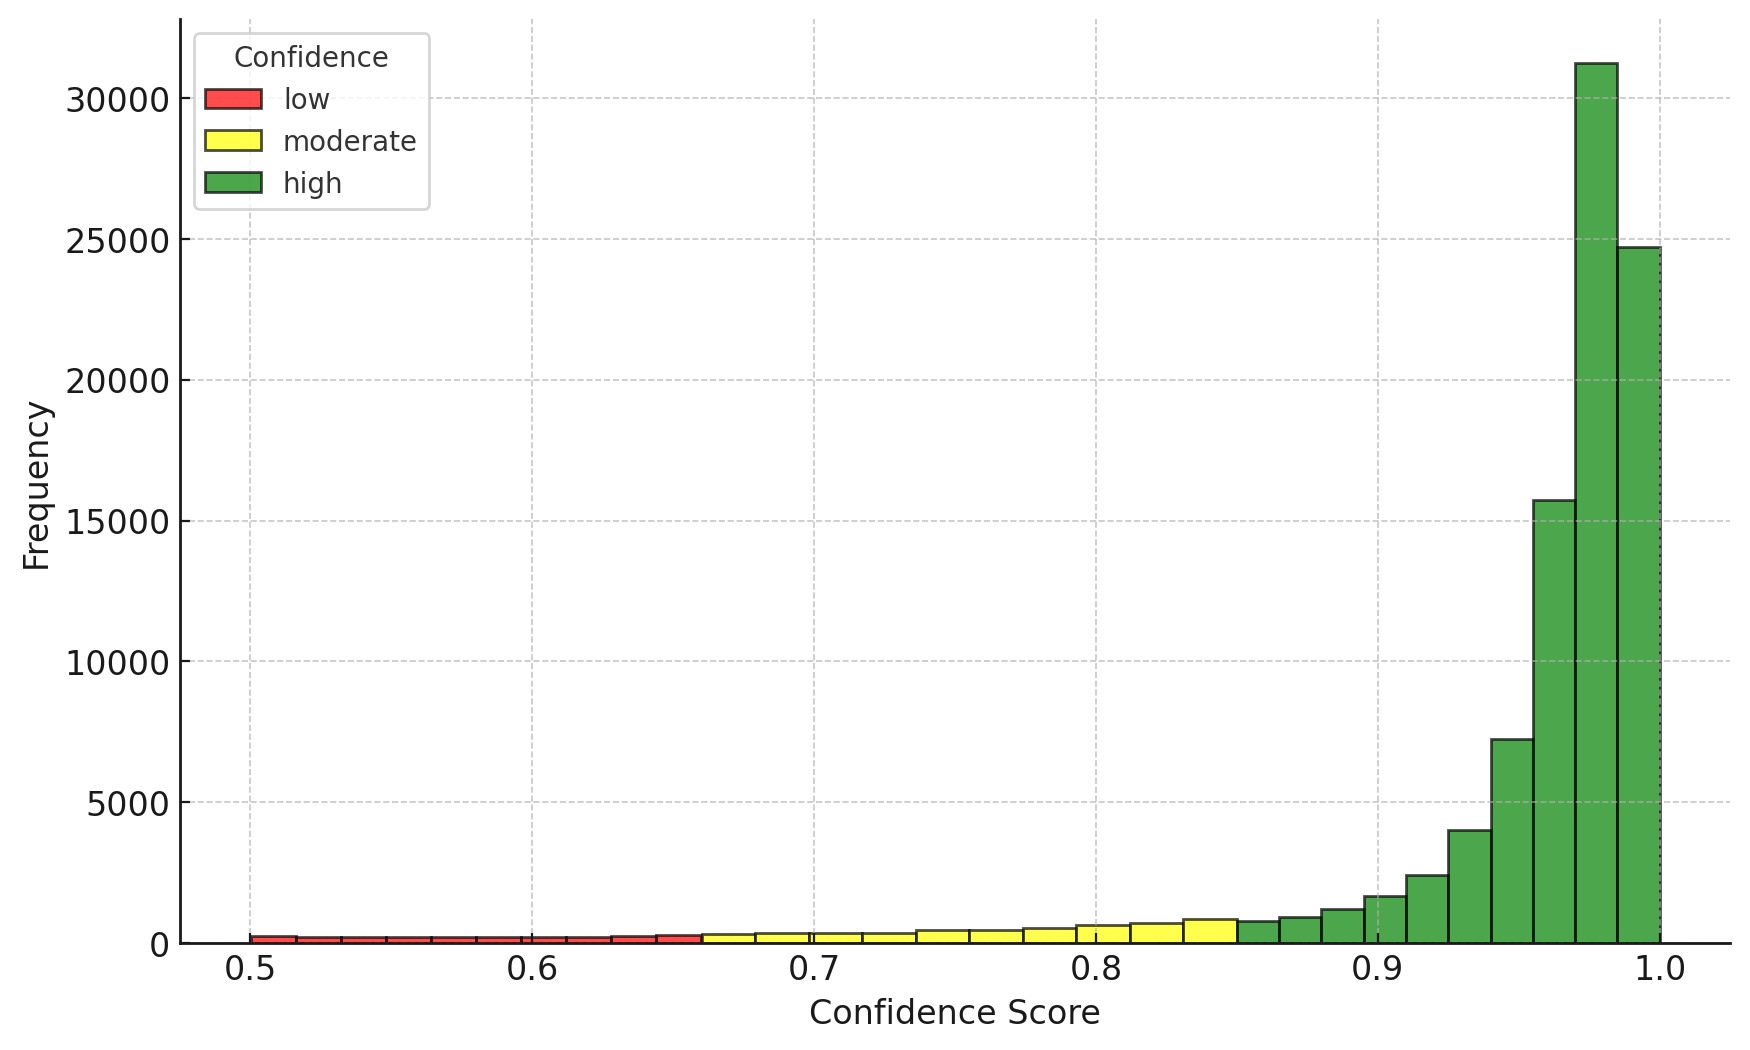
\includegraphics[width=\textwidth]{./figures/confidence_baseline.png}
        \caption{Confidence score distribution for SVM}
        \label{fig:confidence_base}
    \end{subfigure}
    \hfill
    \begin{subfigure}[t]{0.45\textwidth}
        \centering
        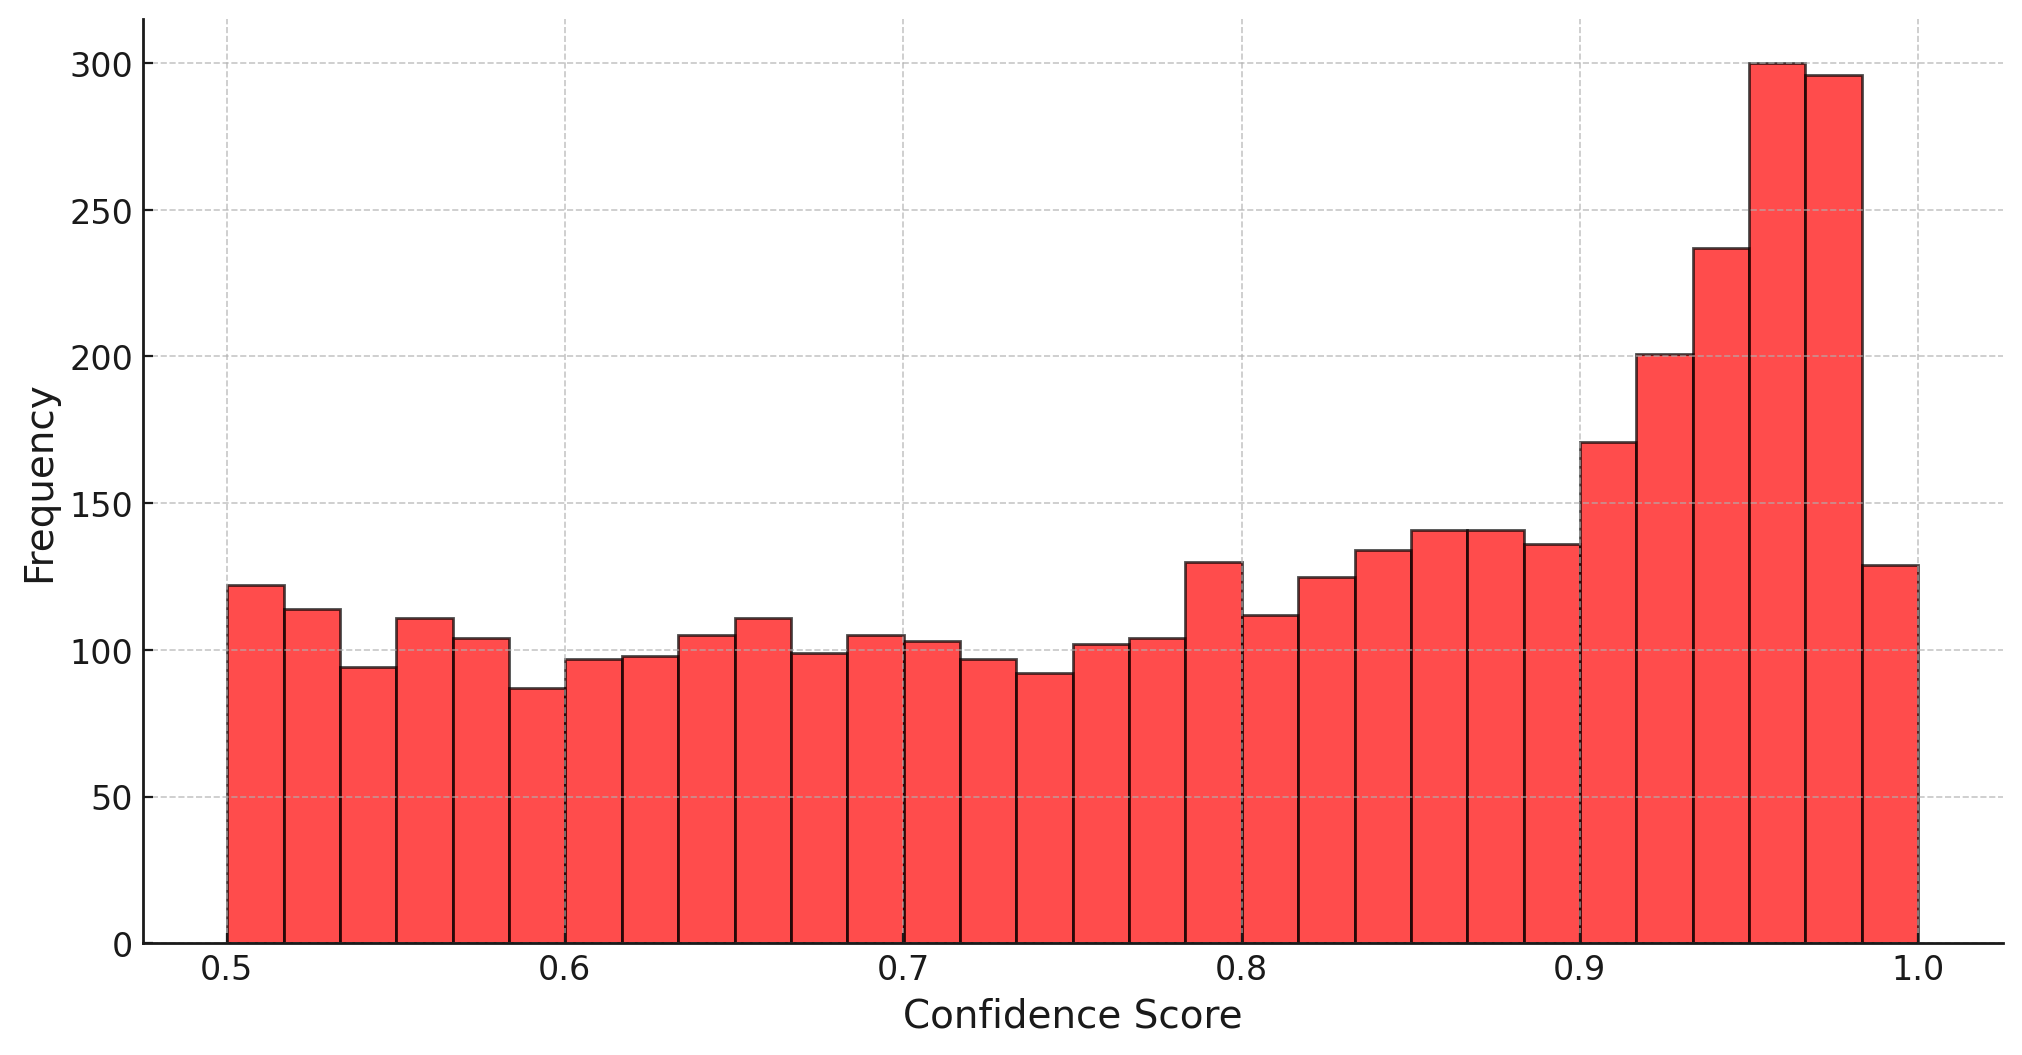
\includegraphics[width=\textwidth]{./figures/wrong_svm.png}
        \caption{Incorrect predictions for SVM}
        \label{fig:incorrect_svm}
    \end{subfigure}

    \vspace{1em}

    \begin{subfigure}[t]{0.45\textwidth}
        \centering
        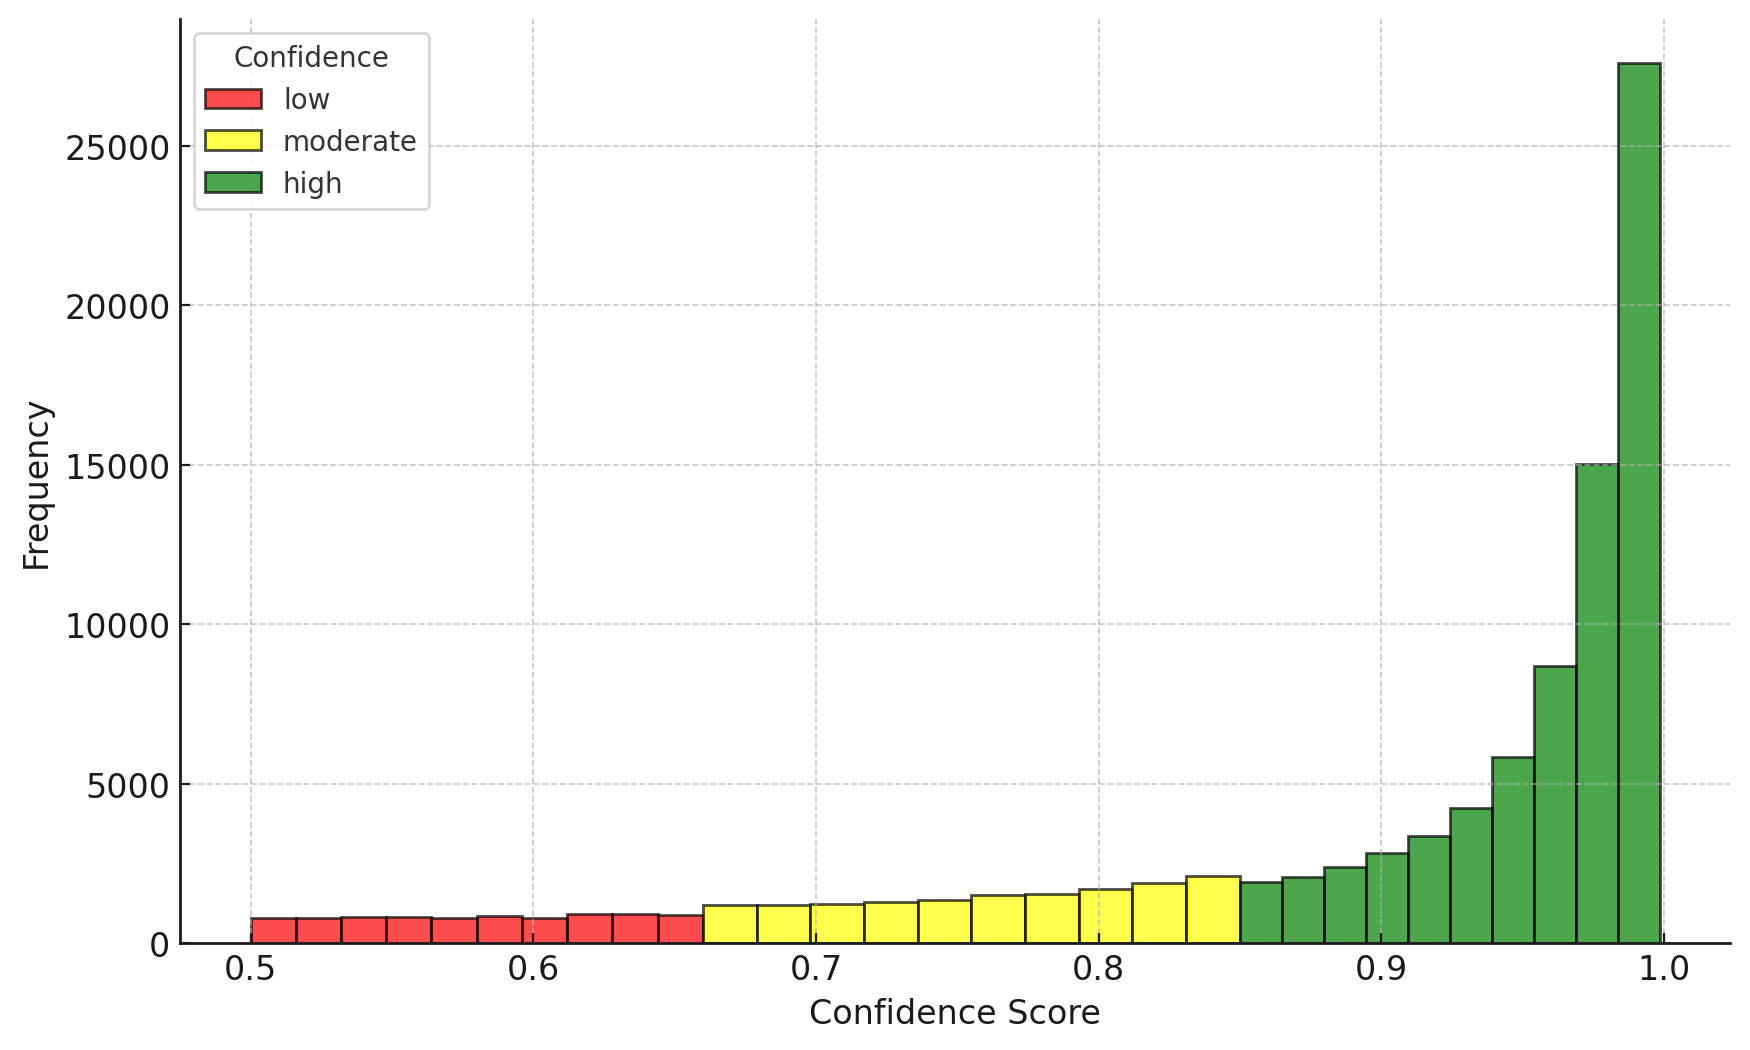
\includegraphics[width=\textwidth]{./figures/confidence_bert.png}
        \caption{Confidence score distribution for BERT}
        \label{fig:confidence_bert}
    \end{subfigure}
    \hfill
    \begin{subfigure}[t]{0.45\textwidth}
        \centering
        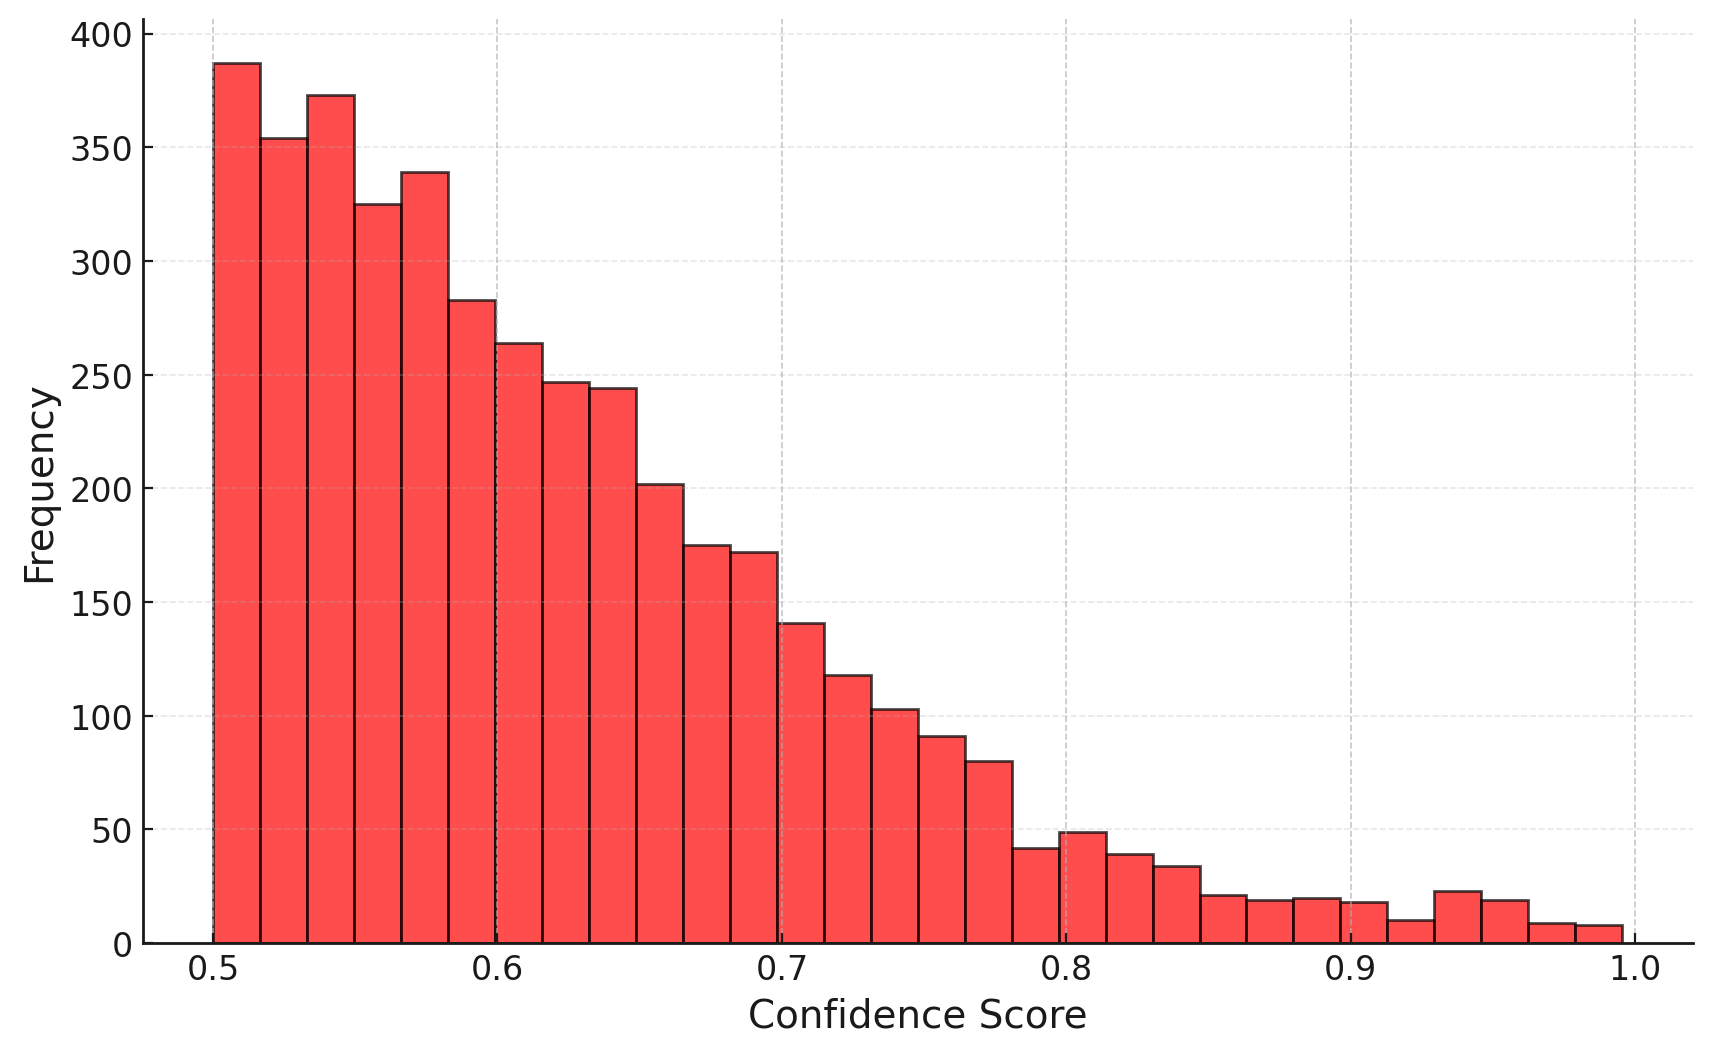
\includegraphics[width=\textwidth]{./figures/wrong_bert.png}
        \caption{Incorrect predictions for BERT}
        \label{fig:incorrect_bert}
    \end{subfigure}

    \caption{Comparison of confidence score distributions and incorrect predictions between SVM and BERT models. Each row represents one model, with the left plot showing confidence score distribution and the right plot showing incorrect predictions.}
    \label{fig:confidence_comparison}
\end{figure}

\section{Example comments}\label{sec:examples}

\begin{table}[htbp]
    \centering
    \caption{False positives with high confidence}
    \label{tab:notable_negative_confidence}
    \scalebox{0.95}{
    \begin{tabular}{p{12cm} c} 
    \toprule
    \textbf{Comment} & \textbf{Confidence Score} \\
    \midrule
    Total Clueless Jerk & 0.8968 \\
    Flat earther moron. & 0.8901 \\
    Damn right & 0.8832 \\
    \bottomrule
    \end{tabular}
    }
\end{table}

\begin{table}[htbp]
    \centering
    \caption{False positives with low confidence}
    \label{tab:fp_low_confidence}
    \scalebox{0.95}{
    \begin{tabular}{p{12cm} c} 
    \toprule
    \textbf{Comment} & \textbf{Confidence Score} \\ 
    \midrule
    The only thing malignant is the rotting flesh between Bernstein's ears. & 0.5000 \\ 
    \midrule
    Calm down. Taking out an airbase is hardly killing millions. It was done tactically perfect. Our troops were not at risk and collateral damage was minimal. Well done and beautiful. He will do things right compared to the loser we had for the past 8 years and the loser that could have been. & 0.5001 \\ 
    \midrule
    garycrum  -  Nice troll post.  Why are you calling me and others in here "Don"? & 0.5002 \\ 
    \bottomrule
    \end{tabular}
    }
\end{table}

\begin{table}[htbp]
    \centering
    \caption{False negatives with high confidence}
    \label{tab:high_confidence_comments}
    \scalebox{0.9}{
    \begin{tabular}{p{14cm} c}
    \toprule
    \textbf{Comment} & \textbf{Confidence Score} \\
    \midrule
    Stupid(:point\_down:) & 0.9954 \\
    \midrule
    Always pleasure GREENLEAF, just google "Plate Climatology Theory", it has only come to the fore-front of research in the last decade or so, there are many articles on it. It's in its infancy, but as it points out, data on this underwater activity with vents and huge volcanoes that truly dwarf those on land, especially the plate faults and their ever releasing not just CO2, but methane and other gases that effect the environment, has been scarce. As you point out, many through history believed their impact to be negligible, but that opinion is being researched, new data gathered and challenged. Our government is very much part of the polarized political debate on climate change, sadly, when opposition presents, it is dismissed often out of hand. We assumed the underwater volcanoes and vents acted a particular way as to be of no concern, they don't throw into the atmosphere thus they don't bring cooling. This damn "CIVIL" format limits me from explaining, it's awful! I'd say more. & 0.9871 \\
    \midrule
    My wife retired as a full-time nursing professor a couple of years ago and her position is now being staffed by several part-timers. The nursing program has been running since the colleges took them over in the 60's and has no signs of slowing down. How is this reacting to market forces? They need experienced full-time staff for the majority of the program delivery and continuity to ensure quality. The reality is that instead these colleges have loaded up management administrators at the expense of front-line teaching staff. The number of these managers has DOUBLED over the past 16 years while the number of faculty members has decreased relative to the number of students in the same period. I estimate that the college system could save \$200 million annually just by going back to the 2001 ratio of management to students. What other organizations have doubled their management staff ratio? It's ridiculous. & 0.9863 \\
    \bottomrule
    \end{tabular}
    }
\end{table}


\begin{table}[htbp]
    \centering
    \caption{False negatives with low confidence}
    \label{tab:fn_low_confidence}
    \scalebox{0.95}{
    \begin{tabular}{p{12cm} c} 
    \toprule
    \textbf{Comment} & \textbf{Confidence Score} \\ 
    \midrule
    Demboski is an embarrassment to Alaskans everywhere. I'm sorry that you had to deal with such blatant bigotry and prejudice, Mr. Jones. Don't let people like Demboski run you out of Alaska. The people of Anchorage have already emphatically rejected her once, it's time to do it again.  
      
    To Ms. Demboski: You are contributing nothing worthwhile to the political and cultural landscape of Alaska. Didn't getting rejected by the people of Anchorage teach you that your brand of nonsense is not welcome here? Do us all a favor and resign. The city and state will be better without you involved in its politics. & 0.5008 \\ 
    \midrule
    Well just how bloody crazy can things get?  
    So, if you're equipped to make a stand-up job of urination - you get to use the men's toilet, otherwise, go sit in the ladies room.  It's really simple, but the liberals want to befog even this! & 0.5008 \\ 
    \midrule
    "She accuses conservatives of being the worst offenders in the misogyny department."  
    McKenna must have forget about Liberal M.P. Nicola Diloria's comment about a conservative M.P. being a stripper.  And Liberal Darshan Kang faces sexual harassment allegations as Liberal M.P.  But no it is those conservatives that are the worst. & 0.5010 \\ 
    \bottomrule
    \end{tabular}
    }
\end{table}
        